
\documentclass[aspectratio=169]{beamer}
\usetheme{Madrid}
\usepackage[citestyle = authoryear]{biblatex}
\bibliography{Bibliography-CBAs-Inflation}
\AtBeginBibliography{\scriptsize}
\usepackage{adjustbox}
\usepackage{color}
% \setbeamertemplate{footline}[frame number]
\title{Bringing Expectations to the Collective Bargaining Table}
\author{Valerie Boctor}
\subtitle{Evidence From Brazilian Firms}
\date{\today}
\usepackage{booktabs}
\begin{document}
	\begin{frame}
	\titlepage
	\end{frame}


	% \begin{frame}
	% \frametitle{Outline}
	% \tableofcontents
	% \end{frame}

	\section{Introduction}
	\begin{frame}
		\frametitle{Motivation}
		\begin{itemize}
			\item Understanding wages and employment during crisis in a high inflation environment
			\item Brazil as a paradigm of emerging economies
			\item Relevance to US: past and present
		\end{itemize}
	\end{frame}

	\begin{frame}
	\frametitle{Main Questions}
		\begin{itemize}
			\item How does the timing of CBAs affect the response of wages and employment to the inflationary news shock?
			\item To what extent do firm-level wages exhibit nominal rigidities and why?
			\item What are the implications of wage and employment behavior in response to the shock for expectations-based monetary policy?
		\end{itemize}
	\end{frame}

	\begin{frame}
	\frametitle{Economic Significance}
		\begin{itemize}
			\item Timing of monetary policy shocks (\cite{oliveiTimingMonetaryPolicy2007})
			\item Nominal rigidities \--- wage adjustment asymmetries (\cite{taylorStayingPowerStaggered2016})
			 \item Real wages \& response of employment (\cite{cardUnexpectedInflationReal1990})
			 \item Monetary policy application: inflation targeting
				\begin{itemize}
					\item Traditional channels are consumption and investment. Analyze potential CBA channel
				\end{itemize}
		\end{itemize}
	\end{frame}

	\section{Background}
		\subsection{The Inflationary News Shock}
			\begin{frame}
				\frametitle{Background I: The Inflationary News Shock}
				\centering
			 	\textbf{Key events: Dual economic and political crises in Brazil 2015 - 2016}
				\begin{enumerate}
					\item \underline{January 2015}: Rousseff begins 2nd term amid allegations of corruption, fiscal malfeasance. Economic recession begins.
					\item \underline{March 2016}: \textbf{Inflationary news shock} \---wave of protests solidifies calls for Rousseff's impeachment
					\item \underline{April 2016}: Rousseff is formally impeached
					\item \underline{May 2016}: Rousseff's powers suspended; V.P. Michel Temer takes over, appoints Ilan Goldfajn Brazilian Central Bank chief.
				\end{enumerate}
			\end{frame}

			\begin{frame}
				\frametitle{Background I: The Inflationary News Shock}
				\centering
				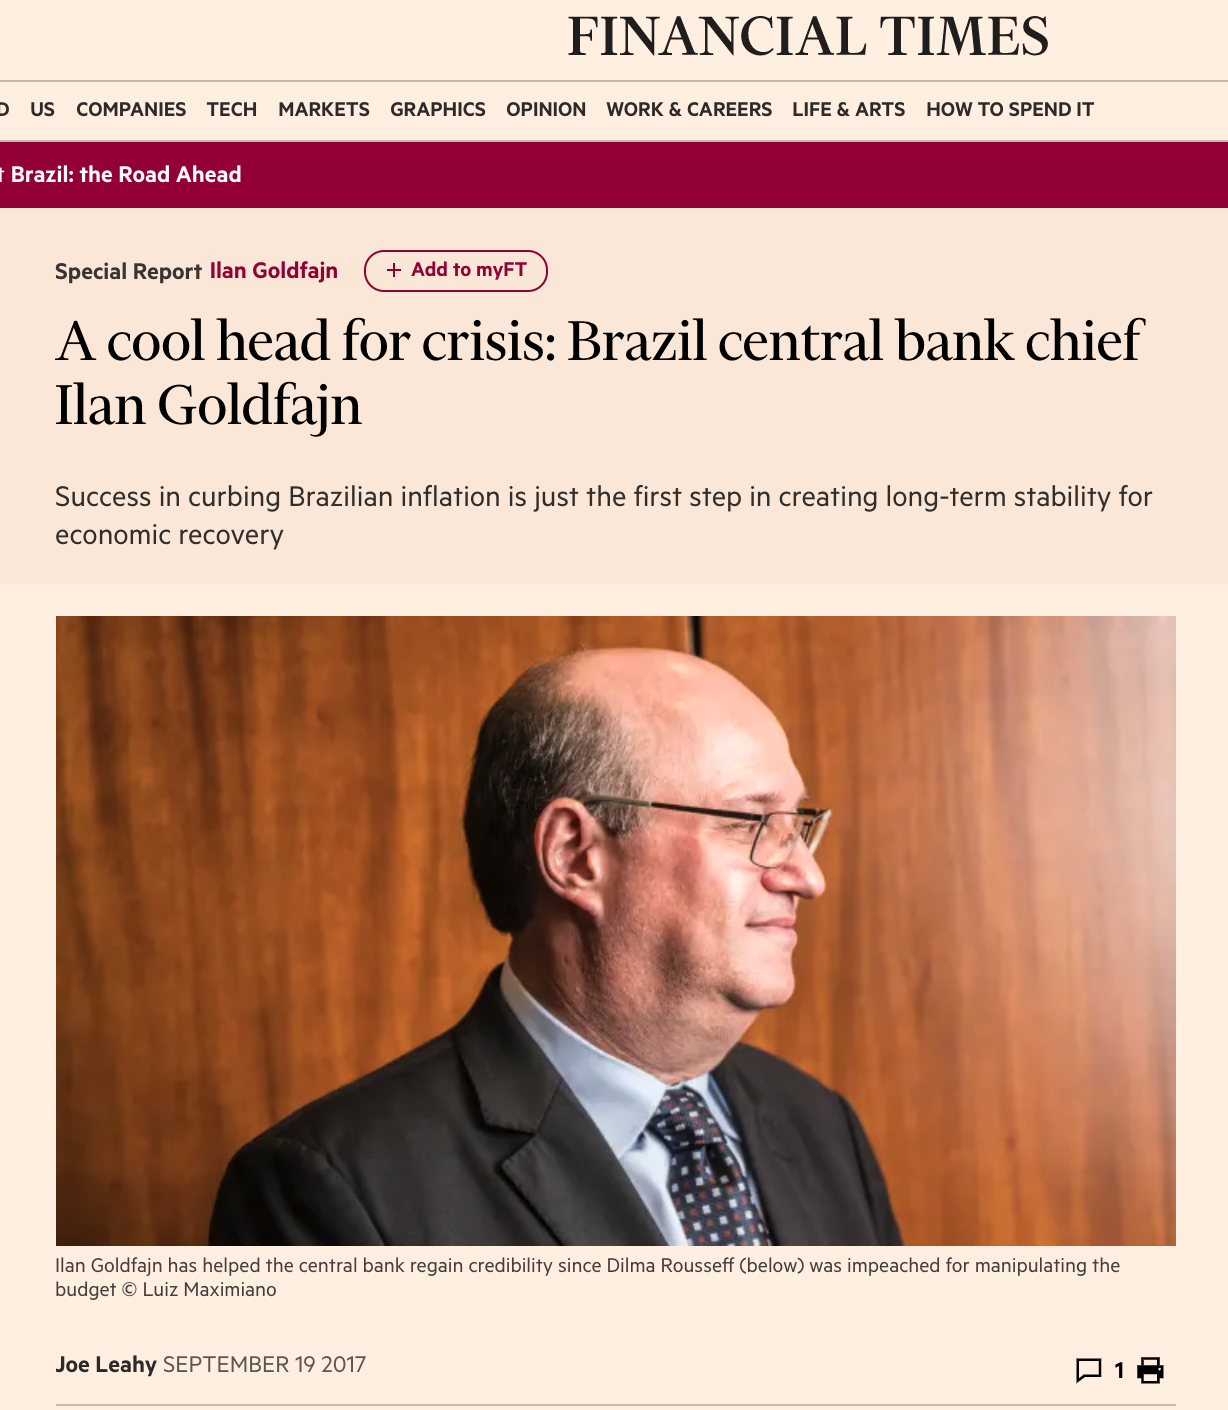
\includegraphics[scale=.3]{old_figures/goldfajn.png}
			\end{frame}	

			\begin{frame}
				\frametitle{Background I: The Inflationary News Shock}
					\centering
					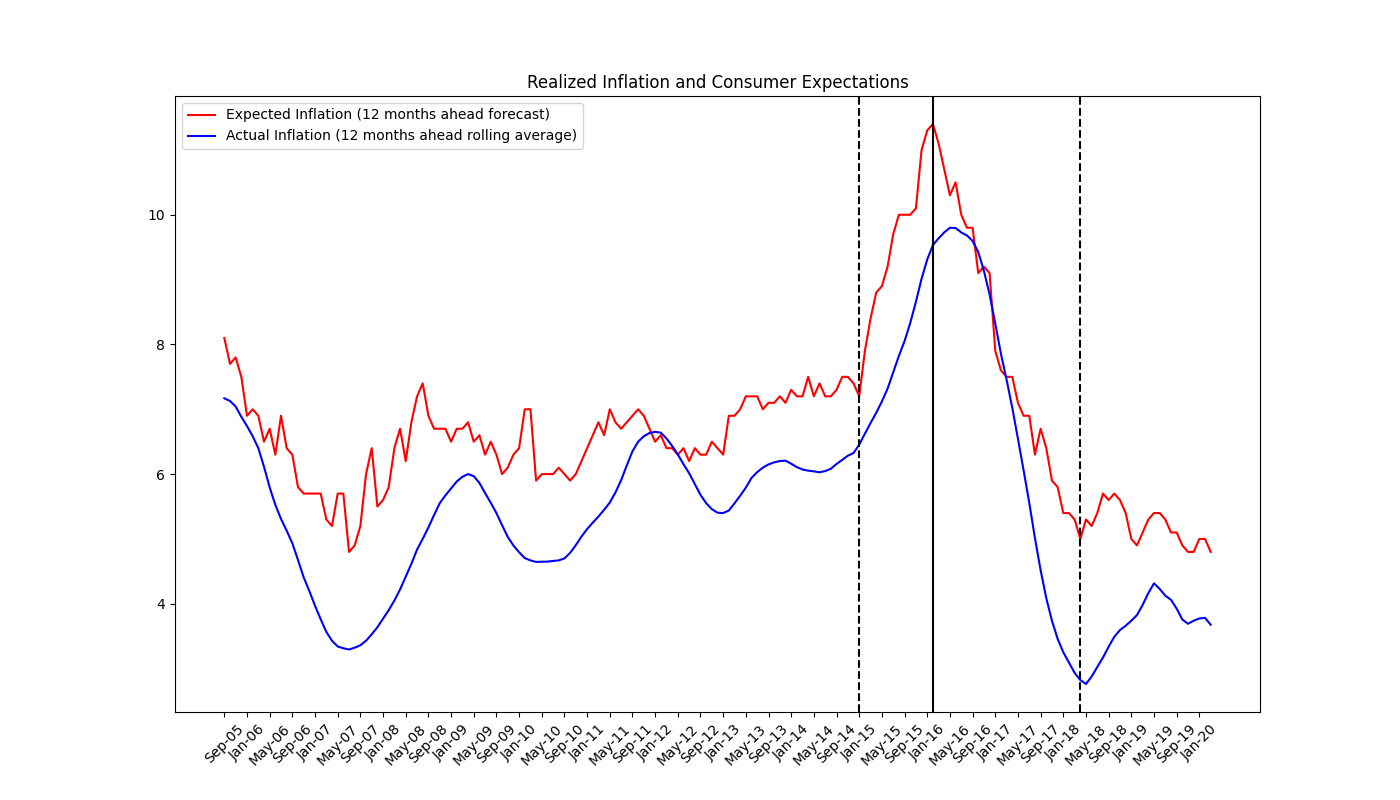
\includegraphics[scale=.35]{tables-figures/Realized_Inflation_and_Consumer_Expectations.png}
			\end{frame}

			\begin{frame}
				\frametitle{Background I: The Inflationary News Shock}
					\centering
					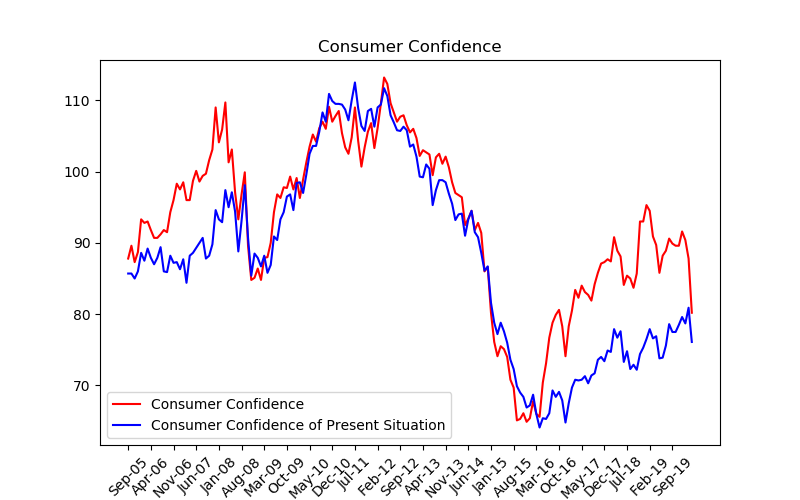
\includegraphics[scale=.55]{old_figures/IBRE_Consumer_Expectations}
			\end{frame}

			\begin{frame}
				\frametitle{Background I: The Inflationary News Shock}
					\centering
					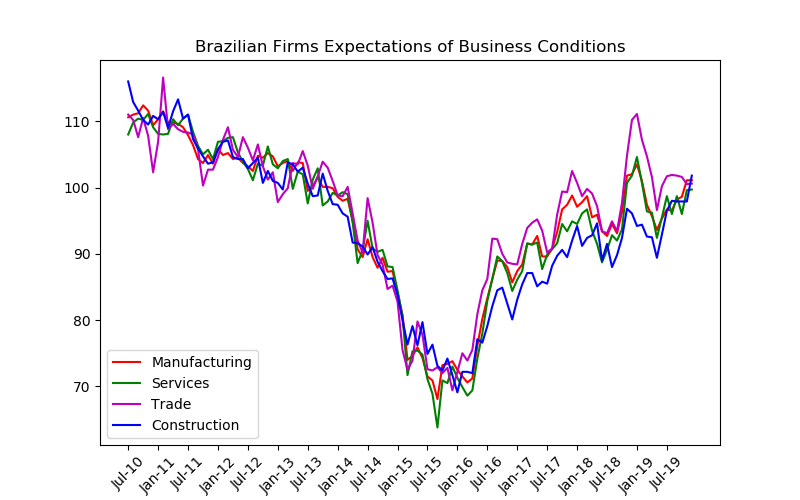
\includegraphics[scale=.55]{old_figures/IBRE_Firm_Expectations}
			\end{frame}
			
		\subsection{CBAs in Brazil}		
			\begin{frame}
				\frametitle{Background II: CBAs in Brazil}
				\begin{itemize}
					\item ~65\% of formal sector workers are unionized in Brazil (compare with ~11\% in US).\cite{byjellevisserTrendsCollectiveBargaining2017}
					\item CBAs typically fix a \textbf{nominal wage level} for the duration of the contract. 
					\item \textbf{Brazilian Consolidation of Labor Laws}: Nominal wages cannot be reduced without workers' approval. 
					\item A reduction in hours must be paired with a commensurate increase in the hourly rate.
					\item Maximum duration of a CBA is 24 months (can be extended indefinitely).
					\item Agreements are either at the firm- or sector- level. We focus on firm-level agreements.
				\end{itemize}
			\end{frame}

			\begin{frame}
				\frametitle{Timing of CBAs in Brazil}
				\begin{center}
				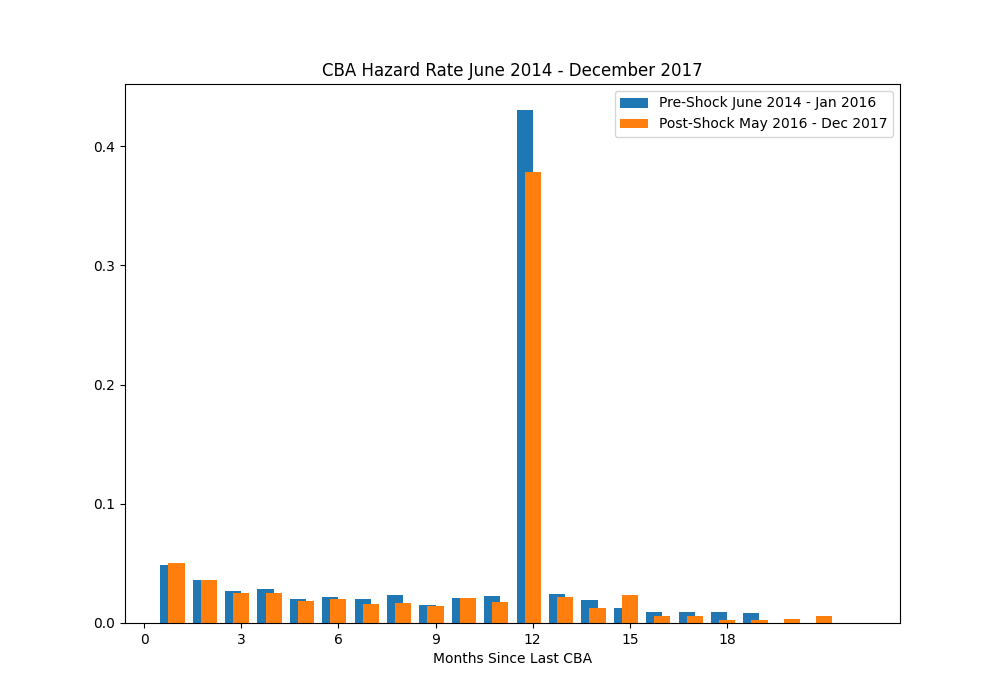
\includegraphics[scale=.45]{tables-figures/cba_hazard.png}
				\end{center}
			\end{frame}

			\begin{frame}
				\frametitle{Timing of CBAs in Brazil}
				\centering
				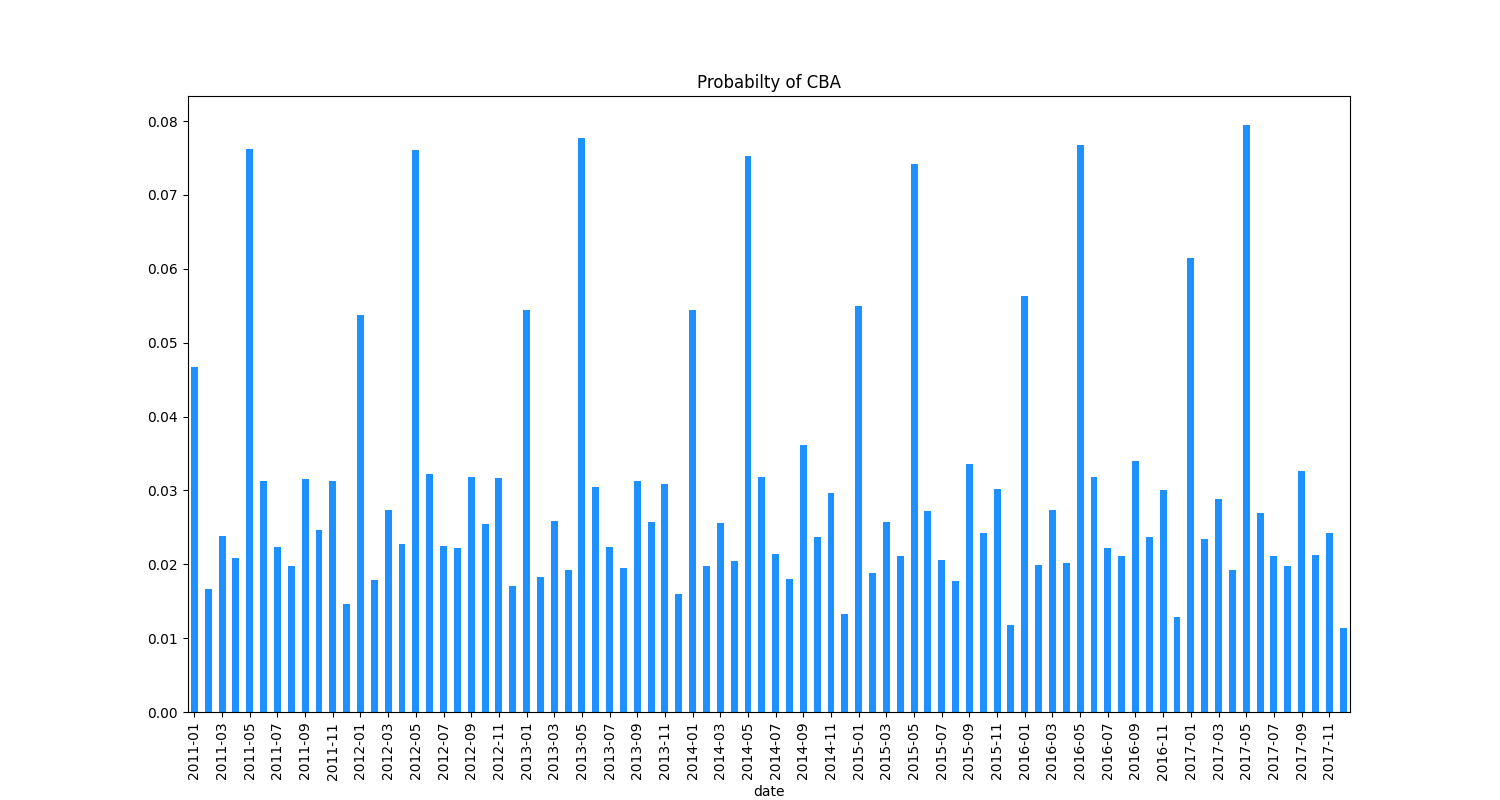
\includegraphics[scale=.35]{tables-figures/cba_probability.png}
			\end{frame}

	\begin{frame}
		\frametitle{Key Takeaways}
		\begin{itemize}
			\item Large drop in inflation expectations coincides with Rousseff's impeachment and  replacement by Temer (and Goldfajn). This represents a plausible inflationary news shock
			\item Variation in the timing of CBAs is plausibly exogenous. 
		\end{itemize}
	\end{frame}

	\section{Data}
		\subsection{RAIS}
		\begin{frame}
			\frametitle{Data}
			\begin{itemize}
				\item \textbf{RAIS} \--- Matched employer-employee data 
				\begin{itemize}
					\item Key variables: Monthly remuneration, employment status, 6-digit occupation code, 2-digit sector code, firm ID, worker ID.
					\item Note: ``Monthly remuneration'' measured observed earnings per worker in a given month. We do not observe wage rates and hours separately.
				\end{itemize}
			\end{itemize}
		\end{frame}

		\subsection{Sistema Mediador}
			\begin{frame}
				\frametitle{Data}
				\label{sistema_mediador}
				\begin{itemize}
					\item \textbf{RAIS} \--- Matched employer-employee data 
					\begin{itemize}
						\item Key variables: Monthly remuneration, employment status, 6-digit occupation code, 2-digit sector code, firm ID, worker ID.
						\item Note: ``Monthly remuneration'' measured observed earnings per worker in a given month. We do not observe wage rates and hours separately.
					\end{itemize}
					\item \textbf{Sistema Mediador} \--- collective bargaining agreements (single firm - employee contracts)
			 		\begin{itemize}
				 		\item Key variables: company names, start/end dates of contracts
					 \end{itemize}
				 \end{itemize}
				 \hyperlink{typical_cba}{\beamerbutton{Example of CBA Contract}}
			 \end{frame}

			 
		\subsection{FGV IBRE}	
			\begin{frame}
				\frametitle{Data}
				\begin{itemize}
					\item \textbf{RAIS} \--- Matched employer-employee data 
					\begin{itemize}
						\item Key variables: Monthly remuneration, employment status, 6-digit occupation code, 2-digit sector code, firm ID, worker ID.
						\item Note: ``Monthly remuneration'' measured observed earnings per worker in a given month. We do not observe wage rates and hours separately.
					\end{itemize}
					\item \textbf{Sistema Mediador} \--- collective bargaining agreements (single firm - employee contracts)
			 		\begin{itemize}
				 		\item Key variables: company names, start/end dates of contracts
					 \end{itemize}
		
				 \hyperlink{typical_CBA}{\beamerbutton{Example of CBA Contract}}
					\item \textbf{FGV IBRE}\--- aggregate inflation expectations	(May gain access to firm-level price and cost expectations)
					\begin{itemize}
						\item Key variables: Aggregate inflation expectations, firm and consumer confidence indices. 
						\item Inflation expectations capture households' projections for inflation over the next 12 months.
					\end{itemize}
				\end{itemize}
			\end{frame}

	\section{Preliminary Findings}

		% \begin{frame}
		% 	\frametitle{Preliminary Results: Real Monthly Remuneration}
		% 	\label{normalized_real_avg_rem}
		% 	% \hyperlink{normalized_a vg_med_rem}{\beamerbutton{Median Plots}}
		% 	\centering
		% 	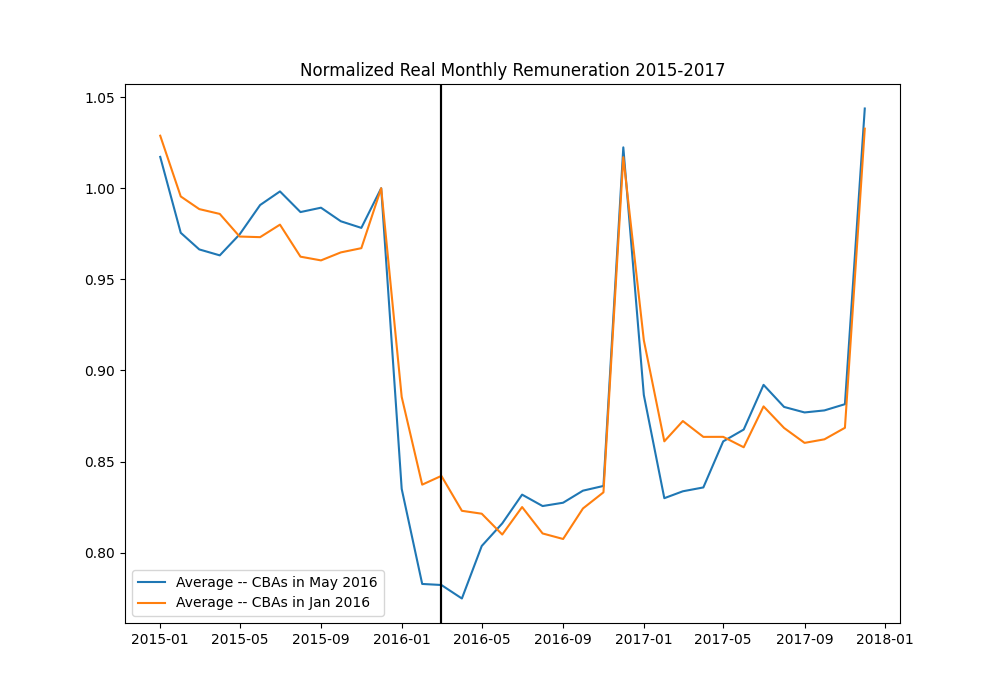
\includegraphics[scale = .4]{tables-figures/normalized_real_avg_rem_2015_2017.png}
		% \end{frame}

		\begin{frame}
			\frametitle{Preliminary Results: Nominal Monthly Remuneration}
			\label{normalized_avg_rem}
			\hyperlink{normalized_avg_med_rem}{\beamerbutton{Median Plots}}
			\centering
			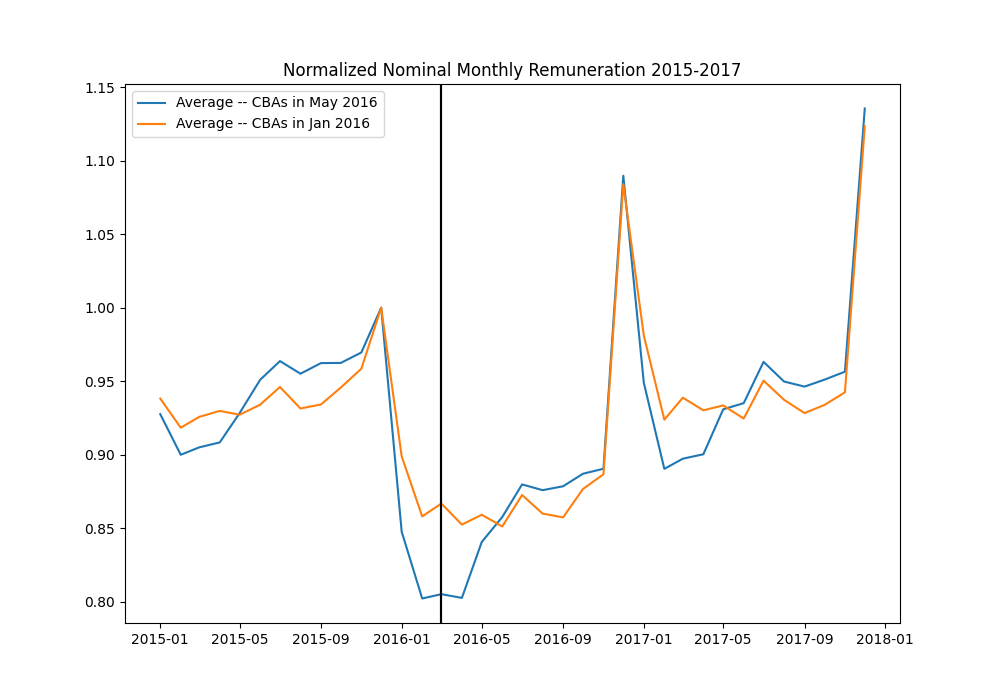
\includegraphics[scale = .4]{tables-figures/normalized_avg_rem_2015_2017.png}
		\end{frame}

		\begin{frame}
			\frametitle{Preliminary Results: Number of Workers}
			\label{normalized_avg_emp}
			\hyperlink{normalized_avg_med_emp}{\beamerbutton{Median Plots}}
			\centering
			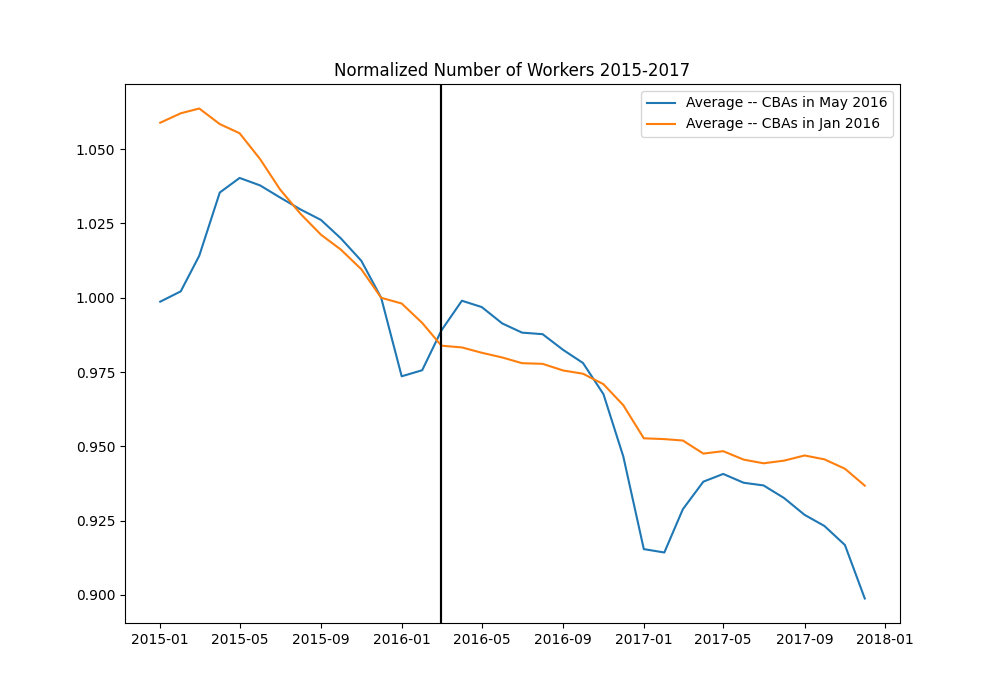
\includegraphics[scale = .4]{tables-figures/normalized_avg_emp_2015_2017.png}
		\end{frame}

		\begin{frame}
			\frametitle{Reduced-Form Model}
		 	Using a DiD approach, we measure effect on CBA timing relative to the shock on nominal wage and employment levels.
			\begin{align}
				\intertext{We write down the reduced form model for wages as:} \label{eqn:rem_DiD}
				\log{w_{i,t}} & = \alpha_i + \delta_t + \sum_{t=\text{Jan 2015}, t\neq t^{\text{shock}}}^{\text{Dec 2017}} \beta_{t}D_{i,t} + \varepsilon_{i,t} 
				\intertext{Similarly, the model for number of workers is:}  \label{eqn:emp_Did}
				\log{n_{i,t}} & = \alpha_i + \delta_t + \sum_{t=\text{Jan 2015}, t\neq t^{\text{shock}}}^{\text{Dec 2017}} \beta_{t}D_{i,t} + \varepsilon_{i,t} 
			\end{align} 

			\begin{itemize}
				\item balanced panel of firms from 2015 - 2017 
				\item contracts set either in Jan 2016 (pre-shock) or May 2016 (post-shock)
			\end{itemize}
		\end{frame}


		\begin{frame}
			\scriptsize{\begin{table}[htbp]\centering
\def\sym#1{\ifmmode^{#1}\else\(^{#1}\)\fi}
\caption{DiD Summary Statistics}
\begin{tabular}{l*{2}{c}}
\hline\hline
            &\multicolumn{2}{c}{postshock\_group}\\
            &           0&           1\\
            &     mean/sd&     mean/sd\\
\hline
num\_workers &     193.650&     142.544\\
            &   (637.540)&   (467.514)\\
rem         &    2786.865&    2236.337\\
            &  (2736.130)&  (1784.036)\\
male        &       0.628&       0.670\\
            &     (0.288)&     (0.305)\\
nonwhite    &       0.357&       0.290\\
            &     (0.333)&     (0.318)\\
lesshs      &       0.245&       0.315\\
            &     (0.262)&     (0.295)\\
hs          &       0.479&       0.486\\
            &     (0.283)&     (0.296)\\
morehs      &       0.276&       0.198\\
            &     (0.308)&     (0.272)\\
\hline
\(N\)       &      510264&            \\
\hline\hline
\end{tabular}
\end{table}
}
		\end{frame}

		\begin{frame}
			\centering
			\begin{table}
				\scriptsize{\begin{tabular}{lrrr}
				 & \multicolumn{3}{c}{postshock\_group} \\
Sector&0&1&Total \\
&\%&\%&\% \\
\hline
Administrative Activities and Ancillary Services&12.6&4.6&8.0 \\
Agriculture&1.4&3.3&2.5 \\
Arts, Culture, Sports and Recreation&0.3&1.1&0.8 \\
Construction&3.0&5.9&4.7 \\
Domestic Services&0.0&0.0&0.0 \\
Education&1.0&1.5&1.3 \\
Electricty and Gas&0.3&0.9&0.6 \\
Extractive Industries&0.8&0.7&0.8 \\
Financial Activities and Insurance&5.4&1.0&2.9 \\
Food and Hospitality&3.3&1.7&2.4 \\
Human Health and Social Services&2.9&4.5&3.8 \\
Information and Communication Technologies&2.3&2.0&2.1 \\
International Organizations&0.0&0.0&0.0 \\
Other Services&7.5&11.2&9.6 \\
Processing Industries&34.1&22.0&27.1 \\
Professional, Scientific, and Technical Activities&2.7&2.1&2.3 \\
Public Administratoin, Defense, and Social Security&0.4&0.8&0.6 \\
Real Estate Activities&1.2&0.2&0.6 \\
Sale and Repair of Motor Vehicles &13.7&17.4&15.8 \\
Transport, Storage and Mail&6.3&18.1&13.1 \\
Water and Waste Management&0.9&1.0&1.0 \\
Total&100.0&100.0&100.0 \\

				\end{tabular}
			}
			\end{table}
		\end{frame}

		\begin{frame}
			\frametitle{DiD Results}
				\centering
				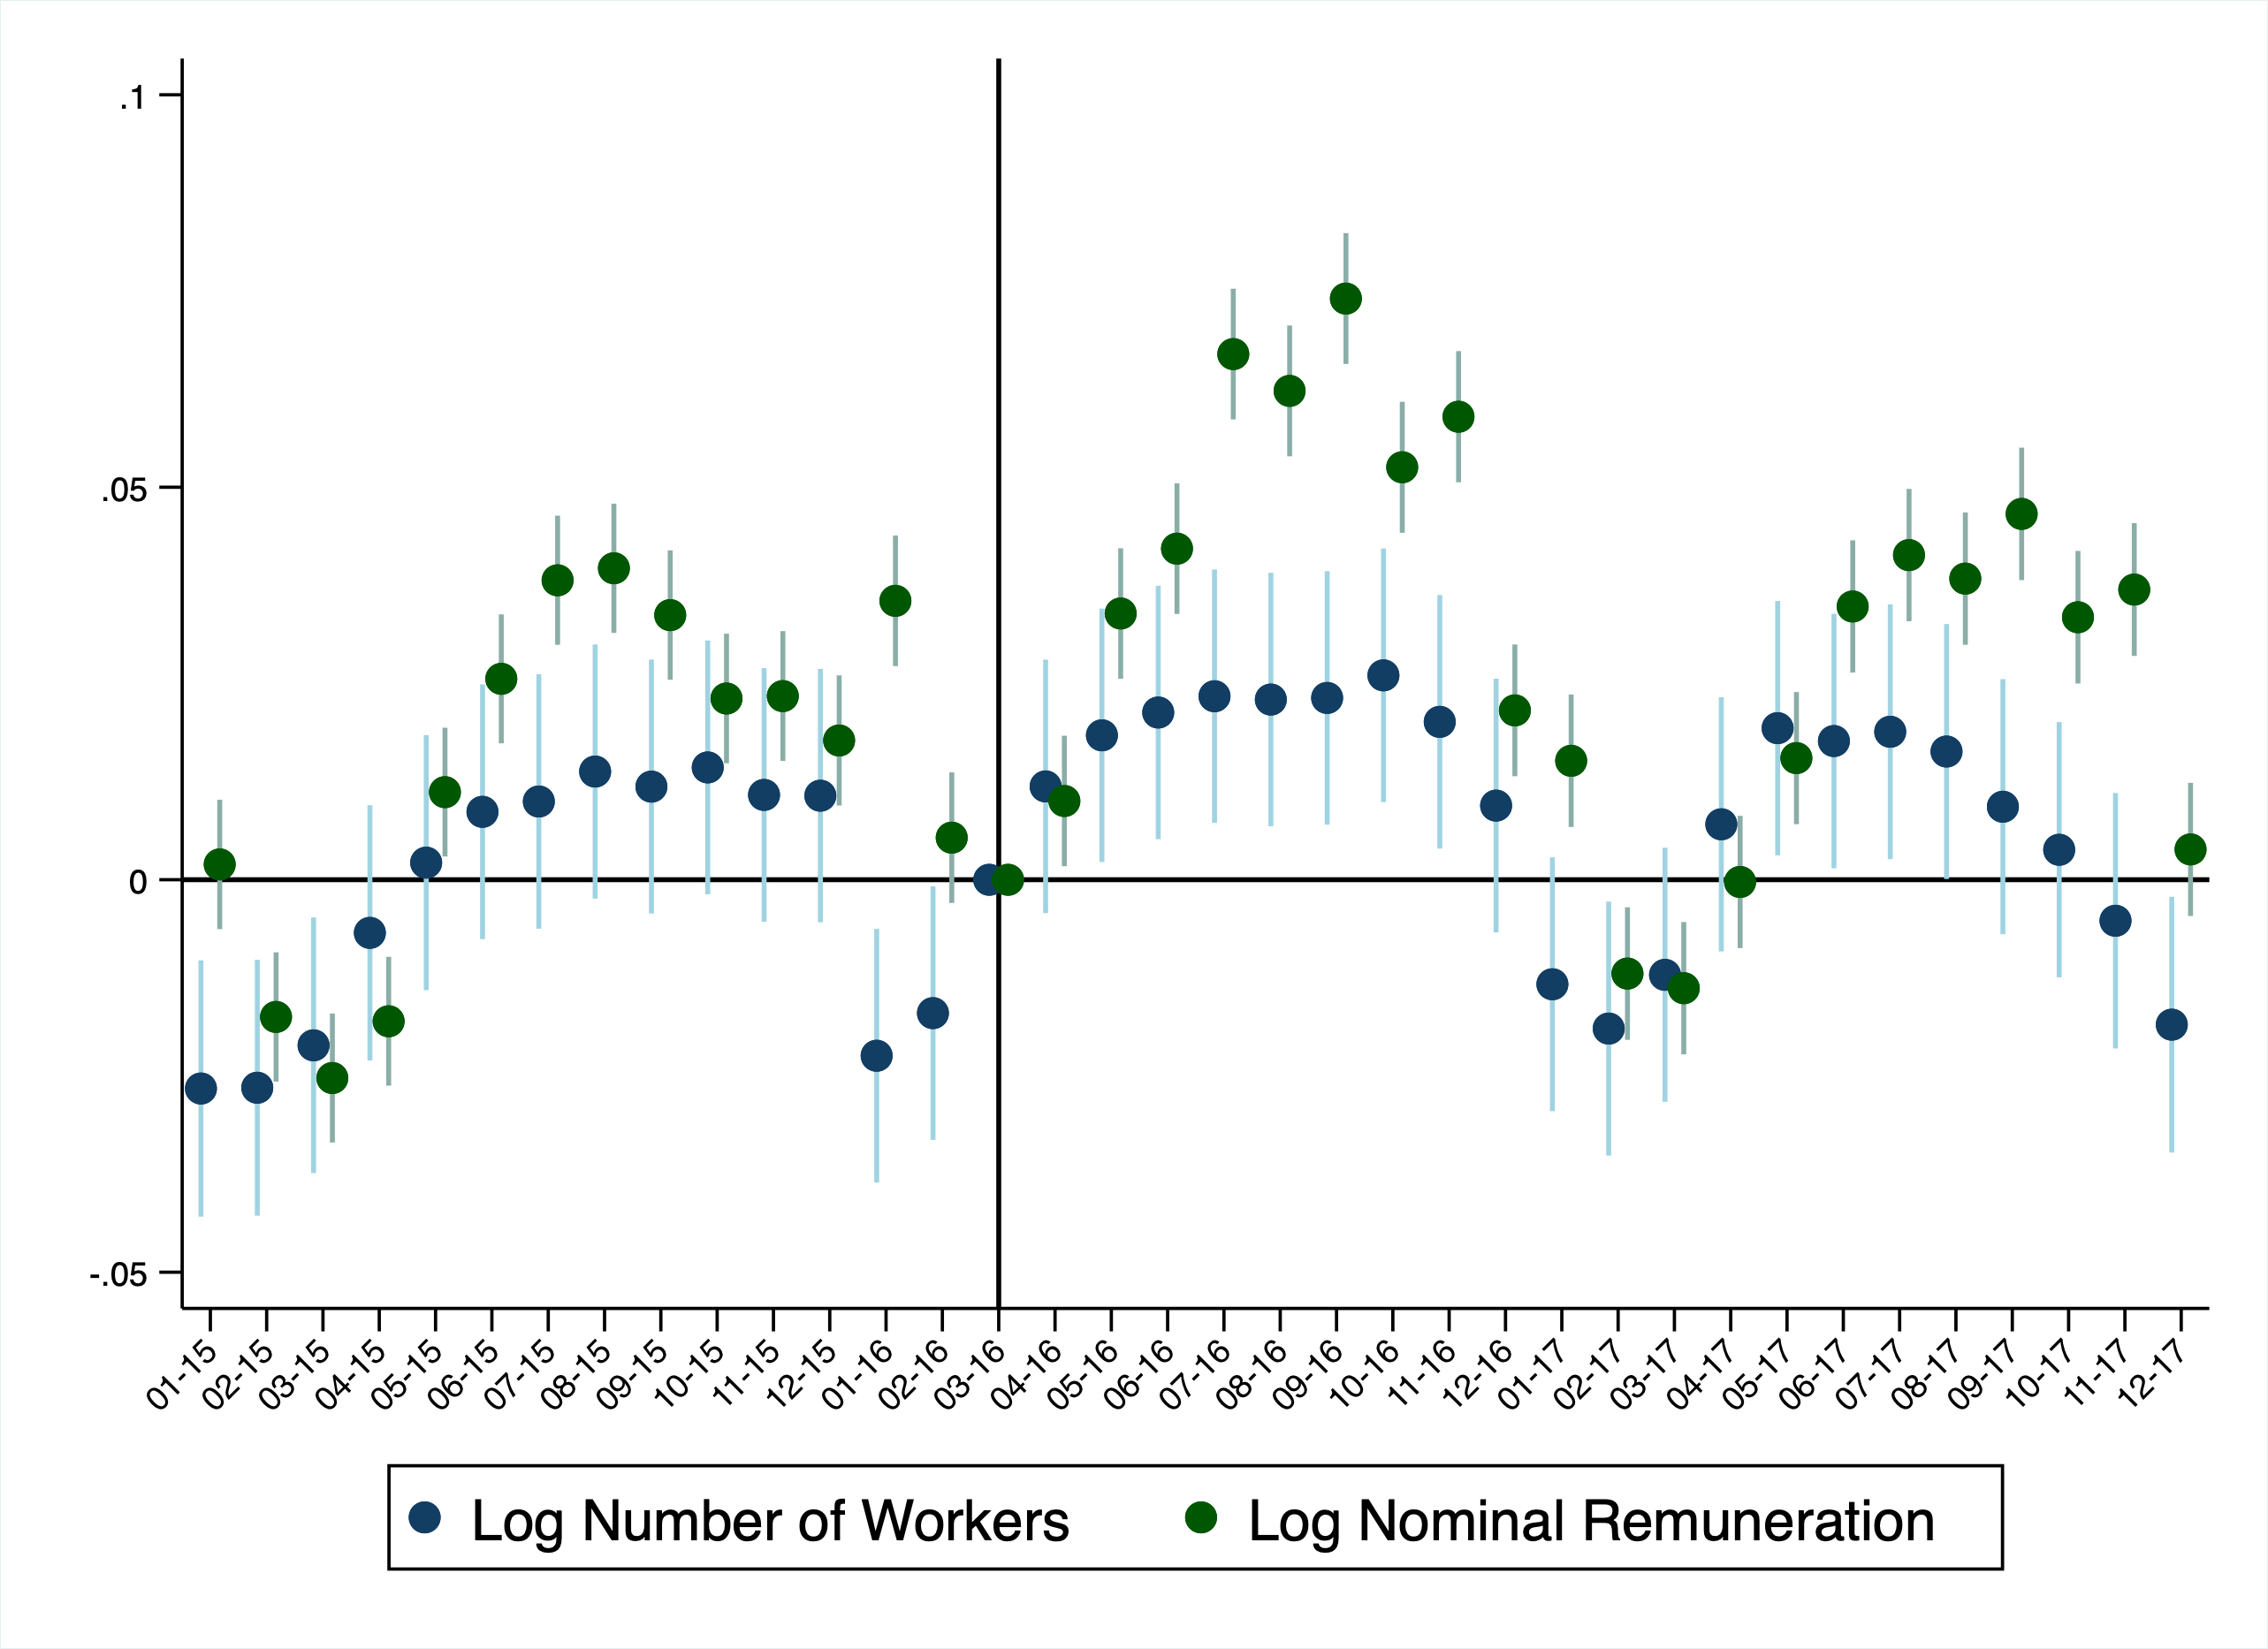
\includegraphics[scale = .225]{tables-figures/DiD_Plots_Weighted_Employment_Rem.png}
		\end{frame}

		\begin{frame}
			\frametitle{Preliminary Findings}
			\begin{itemize}
				\item For both groups of firms, large, persistent drop in nominal wages between Dec. 2015 and Jan. 2016, despite legally-required downward wage rigidity.
				\item This may be driven by mid-month separations, and/or reclassification of workers.
				\item Contrary to prediction, firms with CBAs post-shock actually had higher nominal wages than firms with pre-shock CBAs. 
				\item Seasonality in coefficient estimates
			\end{itemize}
		\end{frame} 

			\begin{frame}
			\frametitle{Preliminary Findings}
			\begin{itemize}
				\item For both groups of firms, large, persistent drop in nominal wages between Dec. 2015 and Jan. 2016, despite legally-required downward wage rigidity.
				\item This may be driven by mid-month separations, and/or reclassification of workers.
				\item Contrary to prediction, firms with CBAs post-shock actually had higher nominal wages than firms with pre-shock CBAs. 
				\item Seasonality in coefficient estimates
			\end{itemize}
			{\color{red}{Possible explanations: optimism, sectoral heterogeneity, cyclicality in workers' bargaining power, regime switching. }}
		\end{frame} 

		\section{Next Steps \& Future Research}
		\begin{frame}
			\frametitle{Next Steps \& Future Research}
			\begin{itemize}
				\item Broaden scope of research question; move beyond inflation shock narrative
				\item Explore heterogeneity across sector
				\item Unpack key drivers in observed nominal wage reduction across groups: separations, reclassifications, or both? 
				\item Estimate effects for real wages and compare with nominal wage and number of workers results.
				\item Pending data access, explore ``optimism'' narrative using own-price/cost expectations microdata. 
				\item Analyze firms' other margins in response to the shock. Data sources?
			\end{itemize}
		\end{frame}
		\begin{frame}
		\frametitle{Structural Identification Strategy}
			\begin{itemize}
				\item Adapt a DSGE model with uneven wage staggering wage model with collective bargaining to assess impacts of monetary policy (\cite{oliveiTimingMonetaryPolicy2007}) or;
				\item Adapt a DMP model with inflation expectations to understand implications for aggregate wages and employment.
			\end{itemize}
		\end{frame}

		\begin{frame}
			\frametitle{References}
			\printbibliography
		\end{frame}

	\section{Additional Projects}
		\begin{frame}
			\centering
			\Huge{Additional Projects}
		\end{frame}

		\begin{frame}
			\frametitle{Regional Inflation Expectations During Covid \& The Phillips Curve}
			Main questions: 
			\begin{itemize}
				\item How do regional economic conditions \& household characteristics (e.g. employment status) during affect household inflation expectations?
				\item What is the slope of the Phillips curve, measured using the regional inflation expectations data?
			\end{itemize}
		\end{frame}

		\begin{frame}
			\frametitle{Regional Inflation Expectations During Covid \& The Phillips Curve}
			\centering
			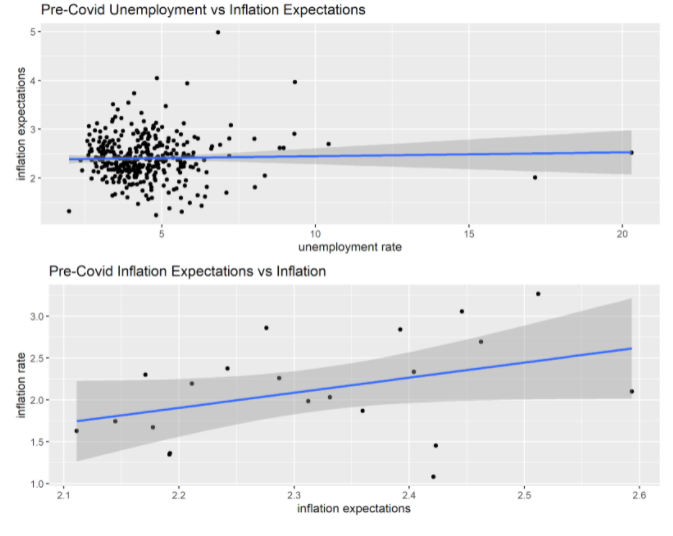
\includegraphics[scale=.35]{tables-figures/Pre-Covid.png}
		\end{frame}

		\begin{frame}
			\frametitle{Regional Inflation Expectations During Covid \& The Phillips Curve}
			\centering
			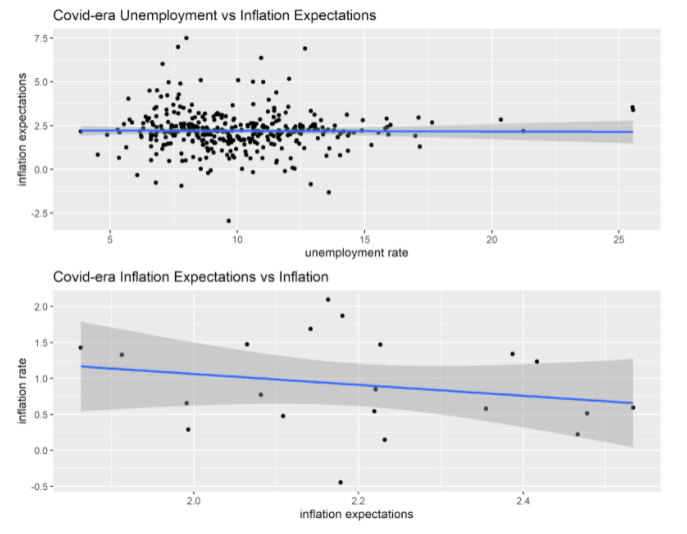
\includegraphics[scale=.35]{tables-figures/Post-Covid.png}
		\end{frame}

		\begin{frame}
			\frametitle{Household Wealth Perceptions and Labor Supply Decisions}
			\begin{itemize}
				\item \textbf{Main question:} How do households' wealth perceptions affect 
				\item i.e., is there a ``Behavioral'' Laffer Curve?
				\item Potential data source: DNB Household Survey
				\item Ideal setting: Look for tax reform as source of exogenous variation in wealth perceptions.
			\end{itemize}
		\end{frame}
	
		\begin{frame}
			\centering
			\Huge{Appendix}
		\end{frame}

		\begin{frame}
			 	\frametitle{Sistema Mediador: Typical CBA (excerpt from \cite{lagosLaborMarketInstitutions2021})}
			 	\label{typical_CBA}
			 	\tiny{Excerpt from (\cite{lagosLaborMarketInstitutions2021})}
				\centering
				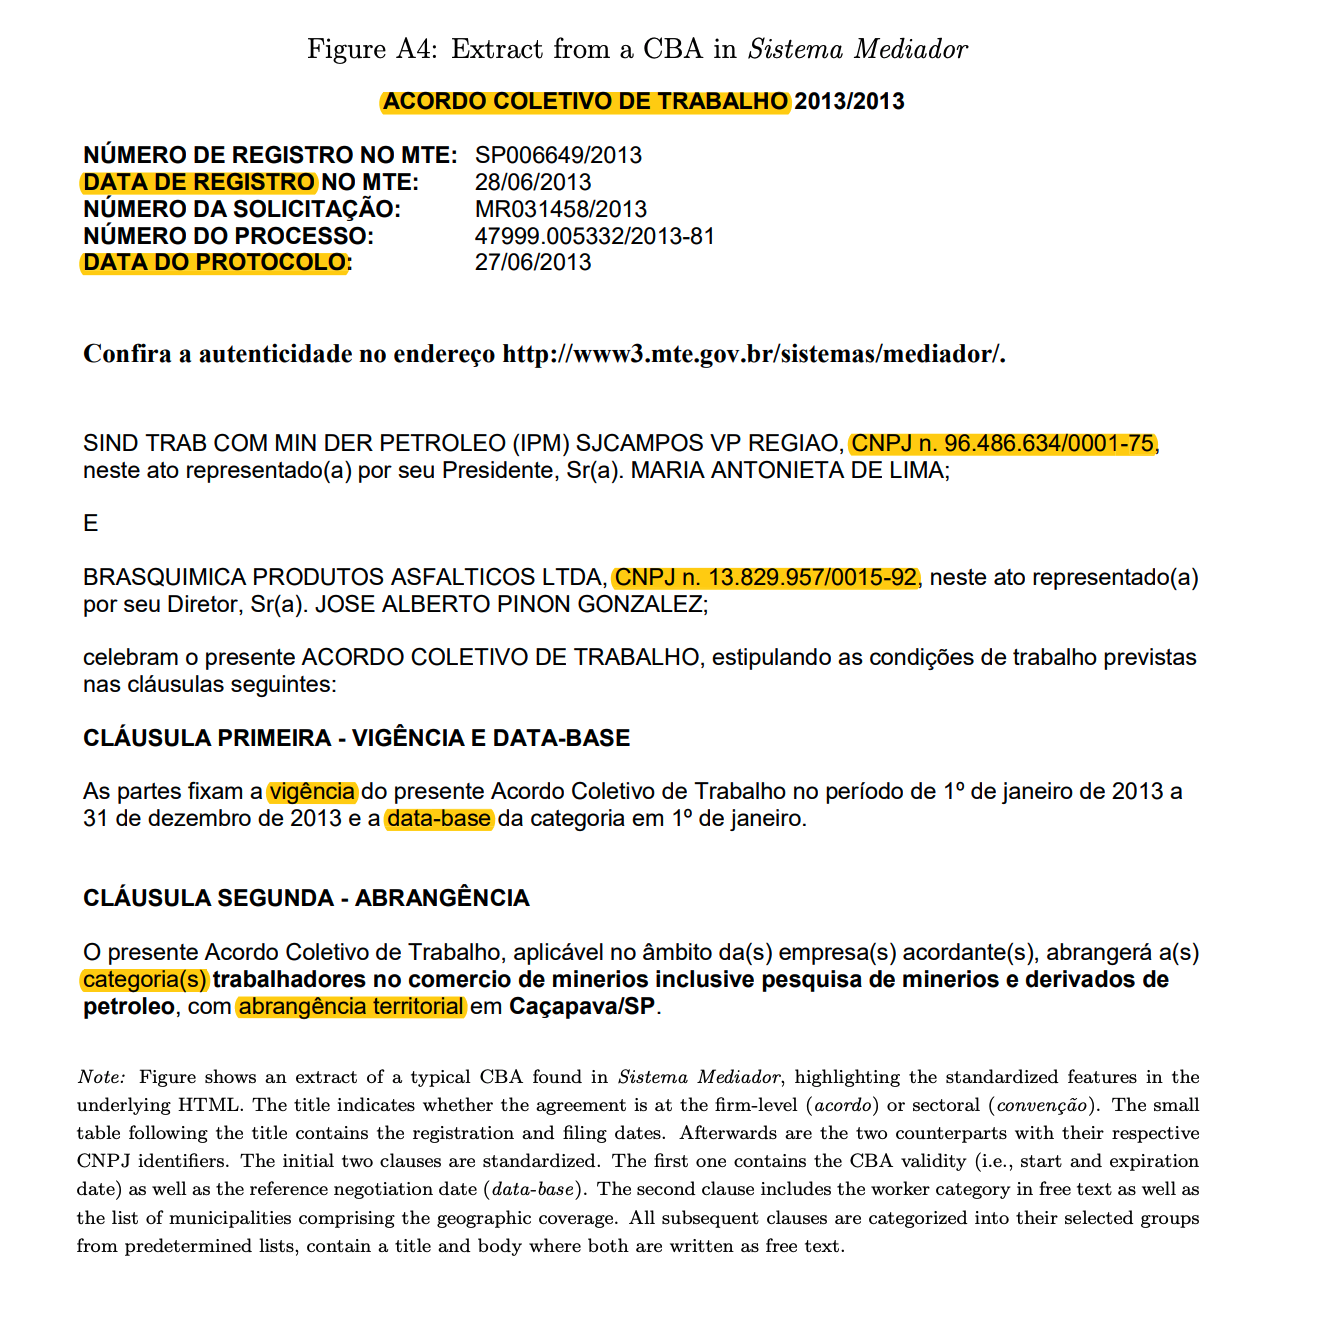
\includegraphics[scale= .3]{tables-figures/Typical_CBA.png}
				\hyperlink{sistema_mediador}{\beamerbutton{Go Back}}
			 \end{frame}

		\begin{frame}
			\frametitle{Preliminary Results: Nominal Monthly Remuneration}
				\label{normalized_avg_med_rem}
				\hyperlink{normalized_avg_rem}{\beamerbutton{Go Back}}
				\centering
				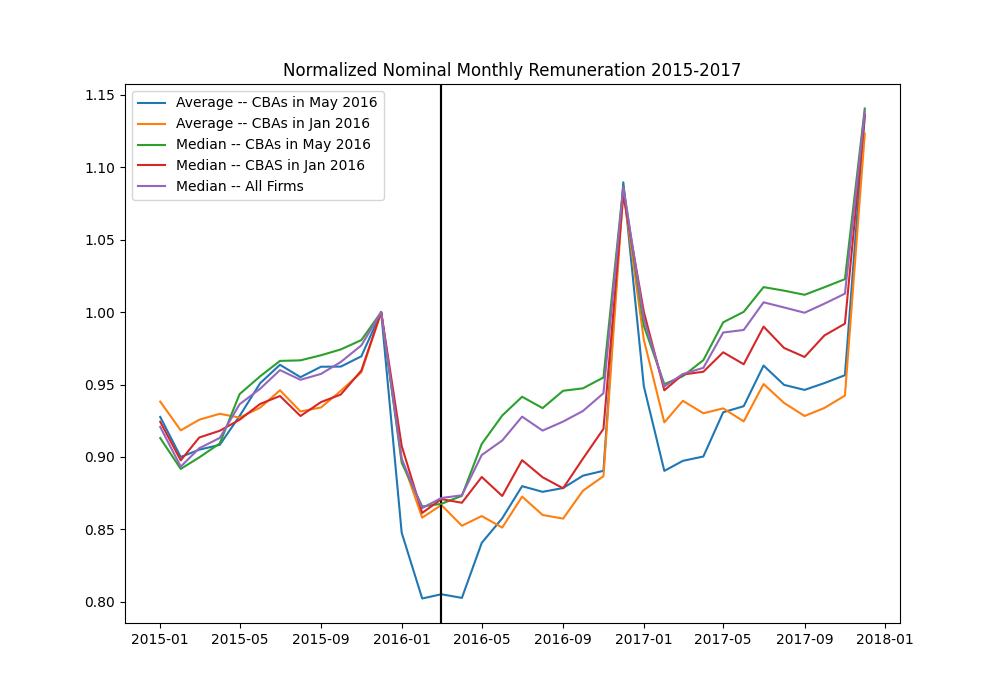
\includegraphics[scale = .4]{tables-figures/normalized_avg_med_rem_2015_2017.png}
		\end{frame}

		\begin{frame}
			\frametitle{Preliminary Results: Number of Workers}
			\label{normalized_avg_med_emp}
			\hyperlink{normalized_avg_emp}{\beamerbutton{Go Back}}
			\centering
			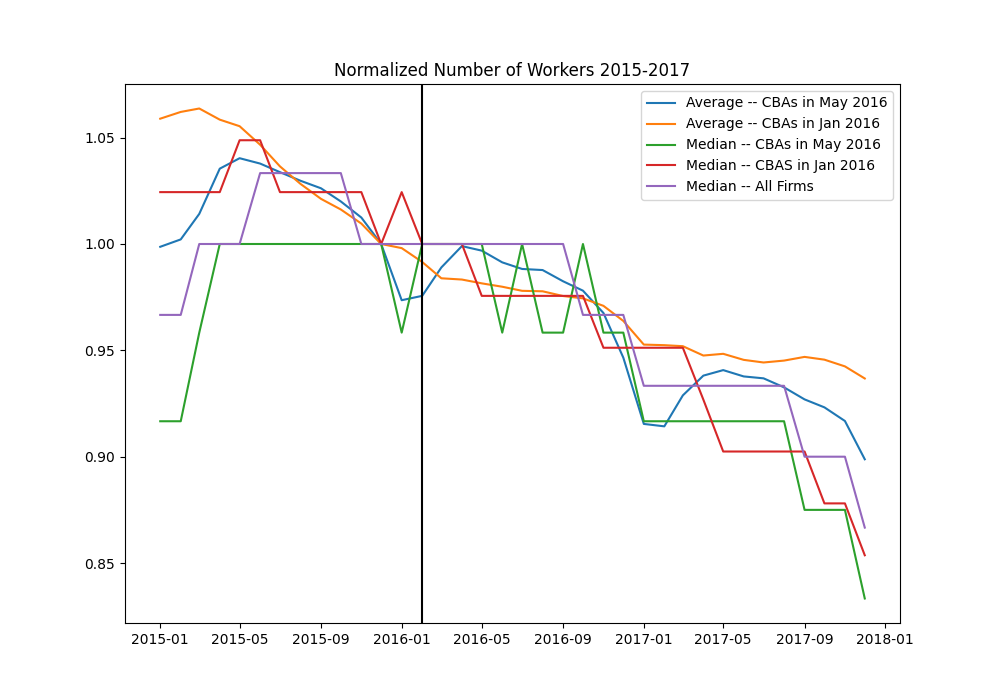
\includegraphics[scale = .4]{tables-figures/normalized_avg_med_emp_2015_2017.png}
		\end{frame}

	\end{document}